
\begin{TP}[Écriture décimale illimitée périodique]

\partie{Écriture décimale illimitée}
\begin{enumerate}
 \item En vous partageant le travail, posez et effectuez les divisions de 5 par 7 et de 8 par 13. Pour chaque quotient, recherchez les dix premières décimales.
 \item On dit que ces écritures sont périodiques. Comment expliquez‑vous cette appellation ?
 \item Déterminez la période de chacun de ces quotients.
 \item Pour chaque quotient, trouvez le vingtième chiffre de la partie décimale. Trouvez le centième ainsi que le millième.
 \end{enumerate}

\partie{Le premier défi}
Inventez un quotient dont l'écriture décimale est illimitée et périodique. Transmettez‑le à un autre groupe et demandez‑leur de trouver l'un des chiffres de la partie décimale dont vous aurez donné le rang. (Par exemple trouvez le $587^\text{e}$ chiffre)


\partie{À la recherche du quotient}
\begin{enumerate}
 \setcounter{enumi}{4}
 \item Un quotient a pour écriture décimale illimitée et périodique $0,\overline{12}$. La longueur de la période est 2. Vérifiez que $\dfrac{12}{99}$ vaut 0,12. \label{NbsRatio_TP}
 \item Donnez l'écriture décimale illimitée périodique de $\dfrac{781}{999}$ avec la notation vue à la question \ref{NbsRatio_TP}.
 \item Quelle fraction a pour écriture décimale illimitée périodique $0,\overline{365\,4}$ ?
 \end{enumerate}

\partie{Le second défi}
Choisissez trois écritures décimales illimitées périodiques dont la période n'excédera pas quatre chiffres et devra commencer tout de suite après la virgule. \\[0.5em]
Échangez‑les avec un autre groupe et retrouvez les écritures fractionnaires qui correspondent aux nombres que vous avez reçus.

\end{TP}


%%%%%%%%%%%%%%%%%%%%%%%%%%%%%%%%%%%
%%%%%%%%%%%%%%%%%%%%%%%%%%%%%%%%%%%
%MiseEnPage
%%%%%%%%%%%%%%%%%%%%%%%%%%%%%%%%%%%
\vfill
%%%%%%%%%%%%%%%%%%%%%%%%%%%%%%%%%%%
%%%%%%%%%%%%%%%%%%%%%%%%%%%%%%%%%%%


%%%%%%%%%%%%%%%%%%%%%%%%%%%%%%%%%%%%%%%%%%%%%%%%%%%%%%%%%%%%%%%%%%%%%%%%%%%%%%

%\begin{TP}[Dans l'Ancienne Égypte]
%
%Dans l'Ancienne Égypte, l'œil du pharaon était utilisé pour signifier « 1 sur ». \\[0.5em]
%$\dfrac{2}{3}$, $\dfrac{3}{4}$ et $\dfrac{1}{2}$ avaient leur propre signe :
%\vspace{0.5em}

%\begin{center}
%$\dfrac{2}{3}$: 
\includegraphics[width=1cm]{pharaon1} \hfill $\dfrac{3}{4}$ : 
\includegraphics[width=1cm]{pharaon2} \hfill $\dfrac{1}{2}$: 
\includegraphics[width=1cm]{pharaon3}
%\vspace{0.3em} 
%$\dfrac{2}{3}$  & 
\includegraphics[width=1cm]{pharaon1} & $\dfrac{3}{4}$  & 
\includegraphics[width=1cm]{pharaon2} & $\dfrac{1}{2}$ & 
\includegraphics[width=1cm]{pharaon3} \\ \hline

%\begin{ttableau}{\linewidth}{6}
% \hline
% $\dfrac{2}{3}$ & 
\includegraphics[width=1cm]{pharaon1} & $\dfrac{3}{4}$ & 
\includegraphics[width=1cm]{pharaon2} & $\dfrac{1}{2}$ & %
\includegraphics[width=1cm]{pharaon3} \\ \hline
%aa & bb & cc & dd & ee & ff \\ \hline
% \end{ttableau}
% \end{center}

%\begin{enumerate}
% \item Complétez la deuxième ligne du tableau suivant avec les symboles des fractions égyptiennes :
% \begin{center}
% \renewcommand*\tabularxcolumn[1]{>{\centering\arraybackslash}m{#1}}
% \begin{ttableau}{\linewidth}{10}
% \hline
% $\dfrac{1}{3}$ & $\dfrac{1}{4}$ & $\dfrac{1}{5}$ & $\dfrac{1}{6}$ & $\dfrac{1}{7}$ & $\dfrac{1}{8}$ & $\dfrac{1}{10}$ & $\dfrac{1}{12}$ & $\dfrac{1}{14}$ & $\dfrac{1}{15}$ \\\hline
 %%%%%%% & & & & 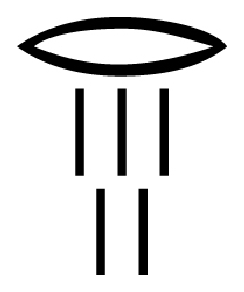
\includegraphics[width=0.7cm]{pharaon4} & & & & & \\ \hline
 %%%%%%% & & 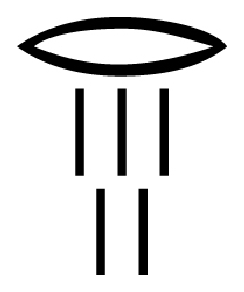
\includegraphics[width=0.7cm]{pharaon4} & & & & 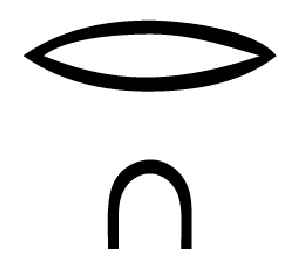
\includegraphics[width=0.7cm]{pharaon5} & & & \\\hline
% \end{ttableau}
 
% \end{center} 
% \item Calculez les sommes suivantes puis donnez leur écriture égyptienne :
 
%\begin{center} $\dfrac{1}{3} + \dfrac{1}{3}$ ; $\dfrac{1}{6} + \dfrac{1}{6}$ ; $\dfrac{1}{3} + \dfrac{1}{6}$ ; $\dfrac{1}{6} + \dfrac{1}{12}$. \end{center}
% \item Pour écrire une fraction, les Égyptiens la décomposaient en une somme de fractions de numérateur 1. Par exemple : $\dfrac{3}{8}$ s'écrivait comme la somme de $\dfrac{1}{4}$ et $\dfrac{1}{8}$ : 
\includegraphics[width=1cm]{pharaon6}  et 
\includegraphics[width=1cm]{pharaon7} \\[0.5em]
%Vérifiez en faisant le calcul.

%À quelles fractions correspondent les écritures suivantes ? \\[0.5em]
%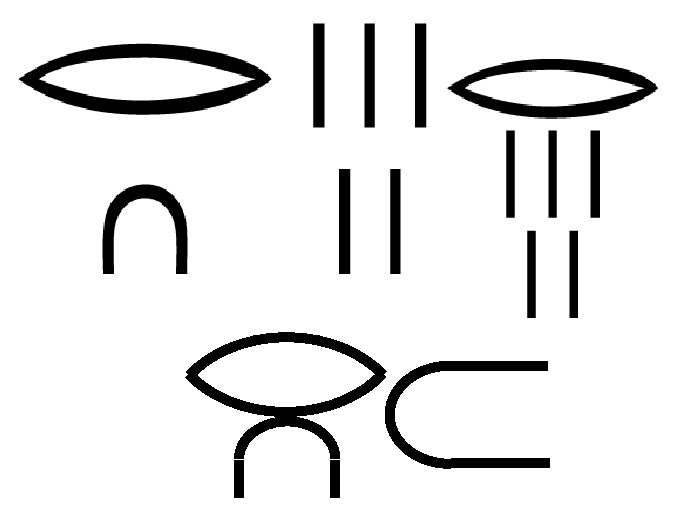
\includegraphics[width=2.3cm]{pharaon_fraction1} \qquad \qquad 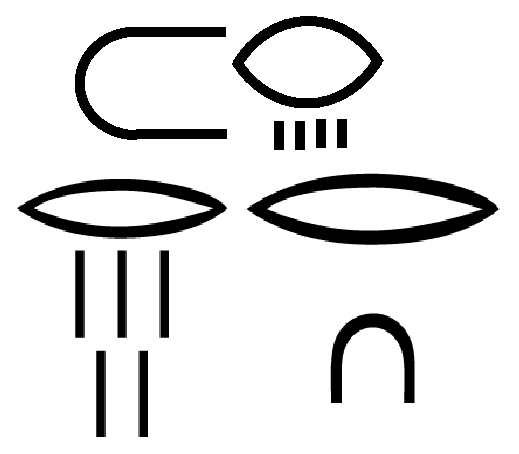
\includegraphics[width=2.1cm]{pharaon_fraction2} \hfill

% \item Inversement, pouvez-vous proposer une écriture égyptienne pour les fractions suivantes ? \\[0.5em]
% $\dfrac{5}{12}$ ; $\dfrac{3}{14}$ ; $\dfrac{7}{12}$ ; $\dfrac{3}{5}$. \\[0.5em]
%La décomposition est-elle toujours unique ?
%\vspace{0.3cm}
% \item Plus difficile !
 
%Pour effectuer le calcul $\dfrac{2}{3} + \dfrac{1}{2}$, le scribe transformait successivement cette somme en $\dfrac{2}{3} + \dfrac{1}{3} + \dfrac{1}{6}$ puis en $1 + \dfrac{1}{6}$ , ce qu'il pouvait alors écrire : \quad 
\includegraphics[width=1cm]{pharaon_fraction3} \\[0.5em]
% \item Faites comme lui pour les sommes : \\[0.5em]
%\begin{center} $\dfrac{2}{3} + \dfrac{2}{3}$ ; $\dfrac{1}{2} + \dfrac{3}{5}$ ; $\dfrac{3}{4} + \dfrac{7}{12}$. \end{center}
% \end{enumerate}

%\end{TP}
